\documentclass[tikz,border=10pt]{standalone}
\usepackage{tikz}
\usetikzlibrary{positioning,arrows.meta,shapes.geometric,shapes.misc,calc}
\begin{document}
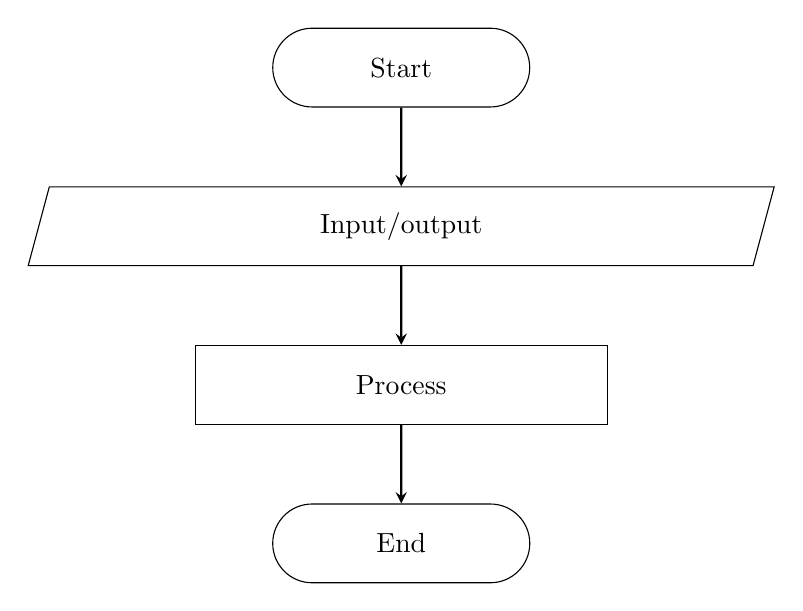
\begin{tikzpicture}[
    node distance=1cm,
    start_end/.style={  
        rounded rectangle,% Rounded rectangle shape  
        draw,  
        text centered,  
        minimum height=1cm,  
        text width=3cm,  
    },  
    process/.style={rectangle, draw, text width=5cm, text centered, minimum height=1cm},
    io/.style={trapezium, trapezium left angle=75, trapezium right angle=105, draw, text width=5cm, minimum width=4.8cm, trapezium stretches=false, text centered, minimum height=1cm},
    arrow/.style={thick, ->, >=stealth}
]
    
    % Nodes
    \node[start_end] (start) {Start};
    \node[io, below=of start] (io) {Input/output};
    \node[process, below=of io] (process) {Process};
    
    \node[start_end, below=of process] (end) {End};
    
    % Connections   
    \draw[arrow] (start) -- (io);
    \draw[arrow] (io) -- (process);
    \draw[arrow] (process) -- (end);
\end{tikzpicture}
\end{document}